\documentclass[twocolumn]{article}
%\documentclass{article}
\usepackage{fullpage}
% you really only need to use one of graphicx or epsfig
% there are example of using each one in this file
%\usepackage[dvips]{graphicx}
%usepackage{epsfig}
\usepackage{pgfplots}

% if you want two columns per page, but you also need to reformat the figures
% to span both columns if you do this
%\twocolumn
\begin{document}
\title{Testing Characteristics of the Linux Page Replacement Policy}

\author{Callen Rain \& Justin Cosentino}

\maketitle

\begin{abstract}
A Brief summary of problem examining and results found
\end{abstract}

\section{Data}
%--------------------------------------------%

\begin{figure*}[t]
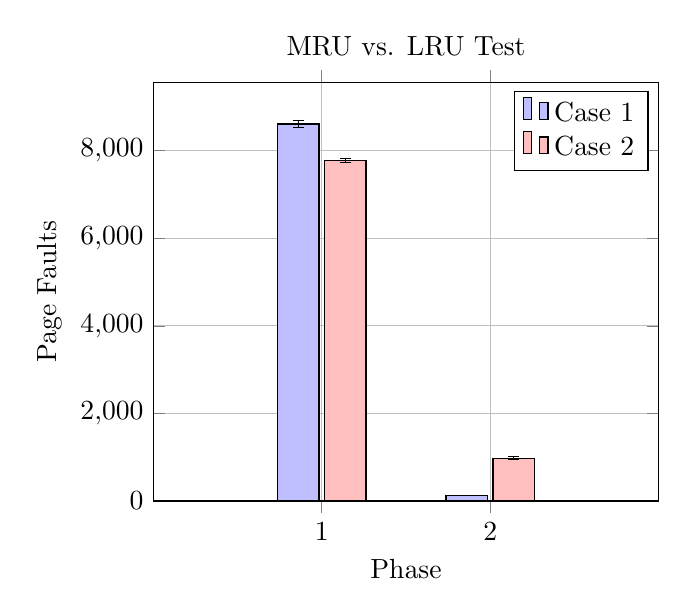
\begin{tikzpicture}
\begin{axis}[
    title = {MRU vs. LRU Test},
    width=8cm,
    xtick={1,...,2},
    xticklabels={1,2,3,4},
    grid=major,
    ybar, 
    bar width=15pt, 
    ylabel=Page Faults, 
    xlabel=Phase, 
    ymin=0, 
        enlarge x limits={abs=1}
    ]

\addplot[
    fill=blue!25,
    error bars/.cd,
        y dir=both,
        y explicit
] 
table [y error=error] {
x   y           error    label
1   8608.00 86.23 1
2   128.00 3.87 2
};

\addplot[
    fill=red!25,
    error bars/.cd,
        y dir=both,
        y explicit
] 
table [y error=error] {
x   y           error    label
1   7775.00   41.76 1
2   978.00   32.60 2
};
\legend{Case 1,Case 2}
\end{axis}
\end{tikzpicture}
\end{figure*}

\begin{table}[h]
\begin{center}
\begin{tabular}{|c|c|r|r|}
\hline
{\bf Phase } & {\bf Case} & {\bf Page Faults} & {\bf Error } \\
\hline
1 & 1 & 8608.00 & $\pm$ 86.23 \\
& 2 & 7775.00 & $\pm$ 41.76 \\
\hline
2 & 1 & 128.00 & $\pm$ 3.87 \\
& 2 & 978.00 & $\pm$ 32.60 \\
\hline
\end{tabular}
\caption{ \label{rawio} MRU versus LRU test data
{\em  Description  }}
\end{center}
\end{table}

%--------------------------------------------%
\begin{figure*}[h]
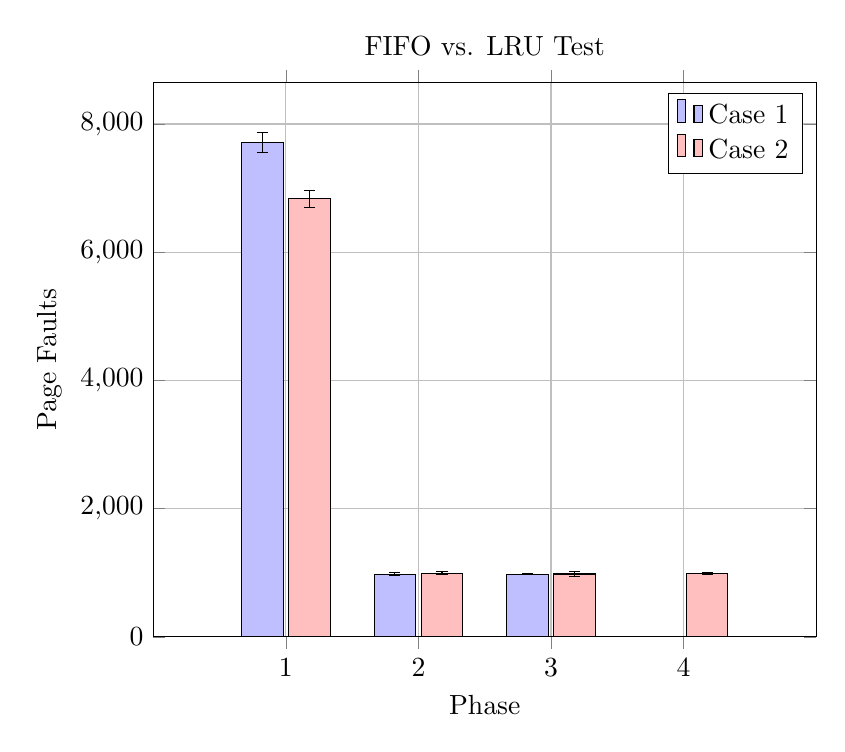
\begin{tikzpicture}
\begin{axis}[
    title = {FIFO vs. LRU Test},
    width=10cm,
    xtick={1,...,4},
    xticklabels={1,2,3,4},
    grid=major,
    ybar, 
    bar width=15pt, 
    ylabel=Page Faults, 
    xlabel=Phase, 
    ymin=0, 
    enlarge x limits={abs=1}
    ]

\addplot[
    fill=blue!25,
    error bars/.cd,
        y dir=both,
        y explicit
] 
table [y error=error] {
x   y           error    label
1   7708.00 158.27 1
2   976.00 20.27 2
3   976.00 8.89 3
4   0.00 0.00 4
};

\addplot[
    fill=red!25,
    error bars/.cd,
        y dir=both,
        y explicit
] 
table [y error=error] {
x   y           error    label
1   6832.00   128.12 1
2   993.00   20.12 2
3   979.00   33.21 3
4   983.00   15.59 4
};
\legend{Case 1,Case 2}
\end{axis}
\end{tikzpicture}
\end{figure*}

\begin{table}[h]
\begin{center}
\begin{tabular}{|c|c|r|r|}
\hline
{\bf Phase } & {\bf Case} & {\bf Page Faults} & {\bf Error } \\
\hline
1 & 1 & 7708.00 & $\pm$ 158.27 \\
& 2 & 6832.00 & $\pm$ 128.12 \\
\hline
1& 1 & 976.00 & $\pm$ 20.27 \\
& 2 & 993.00 & $\pm$ 20.12 \\
\hline
2 & 1 & 976.00 & $\pm$ 8.89 \\
& 2 & 979.00 & $\pm$ 33.21 \\
\hline
1 & 1 & 0.00 & $\pm$ 0.00 \\
& 2 & 983.00 & $\pm$ 15.59 \\
\hline
\end{tabular}
\caption{ \label{rawio} FIFO versus LRU test data
{\em  Description  }}
\end{center}
\end{table}

%--------------------------------------------%
\begin{figure*}[h]
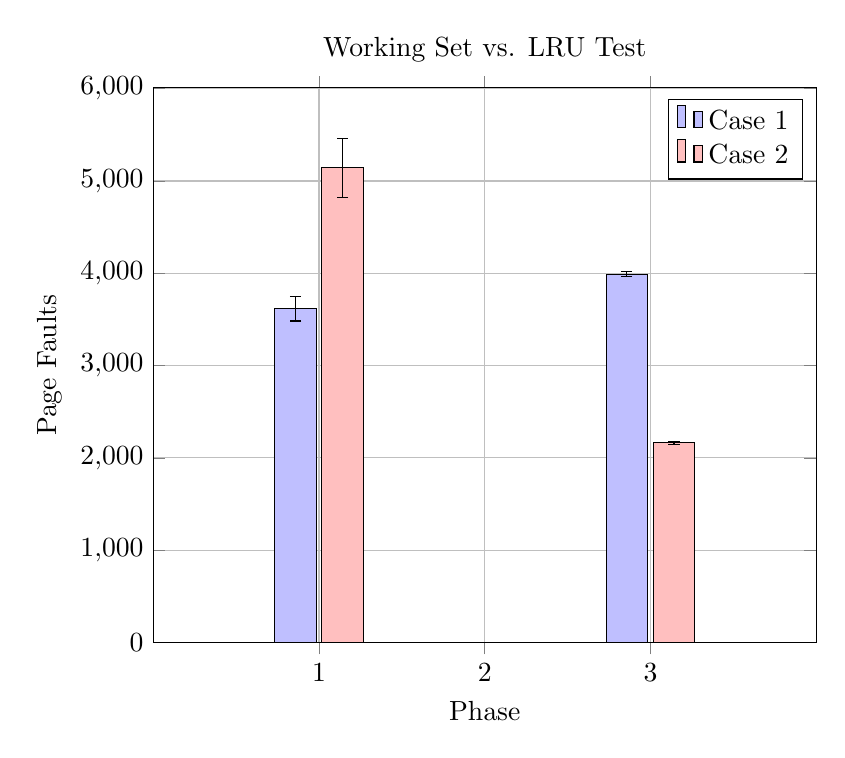
\begin{tikzpicture}
\begin{axis}[
    title = {Working Set vs. LRU Test},
    width=10cm,
    xtick={1,...,3},
    xticklabels={1,2,3,4},
    grid=major,
    ybar, 
    bar width=15pt, 
    ylabel=Page Faults, 
    xlabel=Phase, 
    ymin=0, 
    enlarge x limits={abs=1}
    ]

\addplot[
    fill=blue!25,
    error bars/.cd,
        y dir=both,
        y explicit
] 
table [y error=error] {
x   y           error    label
1   3614.00 131.24 1
2   1.00 1.00 2
3   3990.00 24.58 3
};

\addplot[
    fill=red!25,
    error bars/.cd,
        y dir=both,
        y explicit
] 
table [y error=error] {
x   y           error    label
1   5142.00   320.20 1
2   1.00   0.00 2
3   2163.00   13.96 3
};
\legend{Case 1,Case 2}
\end{axis}
\end{tikzpicture}
\end{figure*}

\begin{table}[h]
\begin{center}
\begin{tabular}{|c|c|r|r|}
\hline
{\bf Phase } & {\bf Case} & {\bf Page Faults} & {\bf Error } \\
\hline
1 & 1 & 3614.00 & $\pm$ 131.24 \\
& 2 & 5142.00 & $\pm$ 320.20 \\
\hline
1& 1 & 1.00 & $\pm$ 1.00 \\
& 2 & 1.00 & $\pm$ 0.00 \\
\hline
2 & 1 & 3990.00 & $\pm$ 24.58 \\
& 2 & 2163.00 & $\pm$ 13.96 \\
\hline
\end{tabular}
\caption{ \label{rawio} Working Set versus LRU test data
{\em  Description  }}
\end{center}
\end{table}

%--------------------------------------------%



\section{Introduction}

Here are some font examples: {\em this is an example of how to get italics fonts } here is {\bf bold} here is a code font {\tt foo(int x);}.

If you want a new paragraph, just put a blank line between the 
current paragraph

and the next paragraph.

\noindent noindent will remove the auto indenting of paragraphs within
a section.

If you want a larger break between paragraphs end the line with slash slash
and add a blank line between it and the next paragraph\\

To refer to a figure tha appears anywhere in the document use 
{\tt backslash ref\{labelname\}} and note where the labelname is defined in
the figure (the tilda glues it to the preceding word of text).
For example: (see Figure~\ref{compvsinterp}). 

Here is an example of how to incorporate a figure in a document...you need
to use one of the psfig or epsfig style files to include a postscript or 
an encapsulated postscript file.  These style files also include macros for
positioning your figure around the text, for changing the size of your figure
for adding captions and labels...  


I can force a figure to the top or bottom of a page by using the [t] or [b].
I can also try to force it to come after the prose it follows in the .tex
file by using [!htb]:



The .cls and .sty files typically contain comments on how to use them in your latex
document...if you look at psfig.sty, the file contains comments that summarize
commands implemented by this style file and how to use them

Here is an example of how to print somthing using a courier font
function \texttt{invokeMethod} while interpreting AP method \texttt{foo}. The 
application program developer wants performance data that measures the



\section {Here is how to create an enumerated list:}

\begin{enumerate}
\item {\bf CPUtime, $<$/APCode/foo.class/foo$>$}:\\
  note the dollar signs around the above are interpreted as math mode.  In
  this mode some characters have special meaning that result in special
  formatting.  Latex is particularly good for representing mathematical
  functions via math mode.  You can also put a large block of text in math
  mode using begin and end. 

\item  The next thing


\item {\bf methodCallTime, $<$/APCode/foo.class/foo$>$}:
  I used to have a mathematical definition for this.
\end{enumerate}


\subsection {Tables in Latex }

Tables are not the easiest interface to use, but you can have latex generate tables for you.
The first part {\tt e.g. |c|l|r|rr|} specifies the number of columns implicitly
and the formating for each column (centered, left, right).  If you put a 
vertical bar between entries, then a vertical bar will be drawn between the
columns otherwise not.  The first example below has 3 columns, the first
uses centered formatting that next two right.  Each row of values is
listed on a separate line.  Ampersands are used between each row's column 
values and backslash-backslah ends a row.   hline can be used to draw
horizontal lines.  multicolumn can be used to span columns and to
change the default column formatting.



Here is a larger example that also demostrates multicolumn directive:




\section {Some random prose to make this longer}

This course is a introduction to the theory, design, and implementation of operating systems. An operating system is the software layer between users and the computer hardware. It implements abstractions that are easier to program than the underlying hardware (e.g. processes, virtual memory, file systems), and it manages the machine's resources (e.g. memory, cpus, disk, network interfaces, and other devices). We will cover the following topics: processes (including synchronization, communication, and scheduling), memory (main memory allocation strategies, virtual memory, and page replacement policies), file systems (including naming and implementation issues), I/O (including devices, drivers, SSDs and disks, and disk scheduling), protection and security, distributed systems and other advanced topics. Prerequisites: CPSC 35 and CPSC 31 required. 

This course is a broad introduction to computer science that focuses on how a computer works and how programs run on computers. We examine the hardware and software components required to go from a program expressed in a high-level programming language like C or Python to the computer actually running the program. This course takes a bottom-up approach to discovering how a computer works, and introduces parallel and distributed computing with a specific focus on parallelism for multicore and other shared memory systems. Topics include theoretical models of computation, data representation, machine organization, assembly and machine code, memory, I/O, the stack, the operating system, compilers and interpreters, processes and threads, and synchronization. In addition to parallel programming, we will discuss parallel computers and system-level support for parallel computing. Prerequisite: Completion of CS21 or its equivalent.

\subsection {Goals for the Course:}

\begin{itemize}
    \item To understand how a sequential or parallel program goes from being expressed in a high-level programming language to being run on the underlying system.
    \item To understand and analyze the systems costs associated with application performance.
    \item To understand the role of the operating system and some of the abstractions it implements to support efficiently running programs.
    \item To understand shared memory parallel computing and to be able to "think in parallel" algorithmically.
    \item To become proficient in using gdb and valgrind to debug and examine program execution state.
    \item To design and implement solutions to large problems using the C programming language.
    \item To design and implement parallel solutions to programming problems that require synchronization using pthreads. 
\end{itemize}



\section{More Random Prose}

This course covers a broad range of topics related to parallel and distributed computing, including parallel and distributed architectures and systems, parallel and distributed programming paradigms, parallel algorithms, and scientific and other applications of parallel and distributed computing. In lecture/discussion sections, students examine both classic results as well as recent research in the field. The lab portion of the course includes programming projects using different programming paradigms, and students will have the opportunity to examine one course topic in depth through an open-ended project of their own choosing. Course topics may include: multi-core, SMP, MMP, client-server, clusters, clouds, grids, peer-to-peer systems, GPU computing, scheduling, scalability, resource discovery and allocation, fault tolerance, security, parallel I/0, sockets, threads, message passing, MPI, RPC, distributed shared memory, data parallel languages, MapReduce, parallel debugging, and applications of parallel and distributed computing.

Class will be run as a combination of lecture and seminar-style discussion. During the discussion based classes, students will read research papers prior to the class meeting that we will discuss in class. During the first part of the course, we will examine different parallel and distributed programming paradigms. During the second part of the course, students will propose and carry out a semester-long research project related to parallel and/or distributed computing. The department's gigabit cluster, two eight processor workstations, as well as the CS lab machines, are available for course projects.

Previous course work in Operating Systems, Networking, Databases, or Architecture is helpful, but not necessary for taking this course. 

\section{Conclusion}

To figure out how to do something in latex, look at some examples and some
on-line documentation, or google for it.  Often times it is very difficult
to get latex to format something differently from what its default formatting
is. 




\end{document}

